\section{Answers to questions}

Before answering these questions, it is good to make a clarification. To obtain these kind of graphs, 
we decided to take as the execution time the average between the execution times of each quartet, that is, 
of the groups of files that shared the same number of vertices.

\subsection{Question 1}
\textit{Run the three algorithms you have implemented (Prim, Kruskal naive and Kruskal efficient) on the 
graphs of the dataset. Measure the execution times of the three algorithms and create a graph showing the 
increase of execution times as the number of vertices in the graph increases. Compare the measured times 
with the asymptotic complexity of the algorithms. For each problem instance, report the weight of the minimum 
spanning tree obtained by your code.} \\

\noindent
We have implemented the code in C\# for the execution of the three algorithms on the whole provided dataset. 
The results, which have been reported in detail and with the relative weights also in the appendix section, 
are shown below.

\subsubsection{Results of Prim}
\begin{figure}[H]
    \centering
    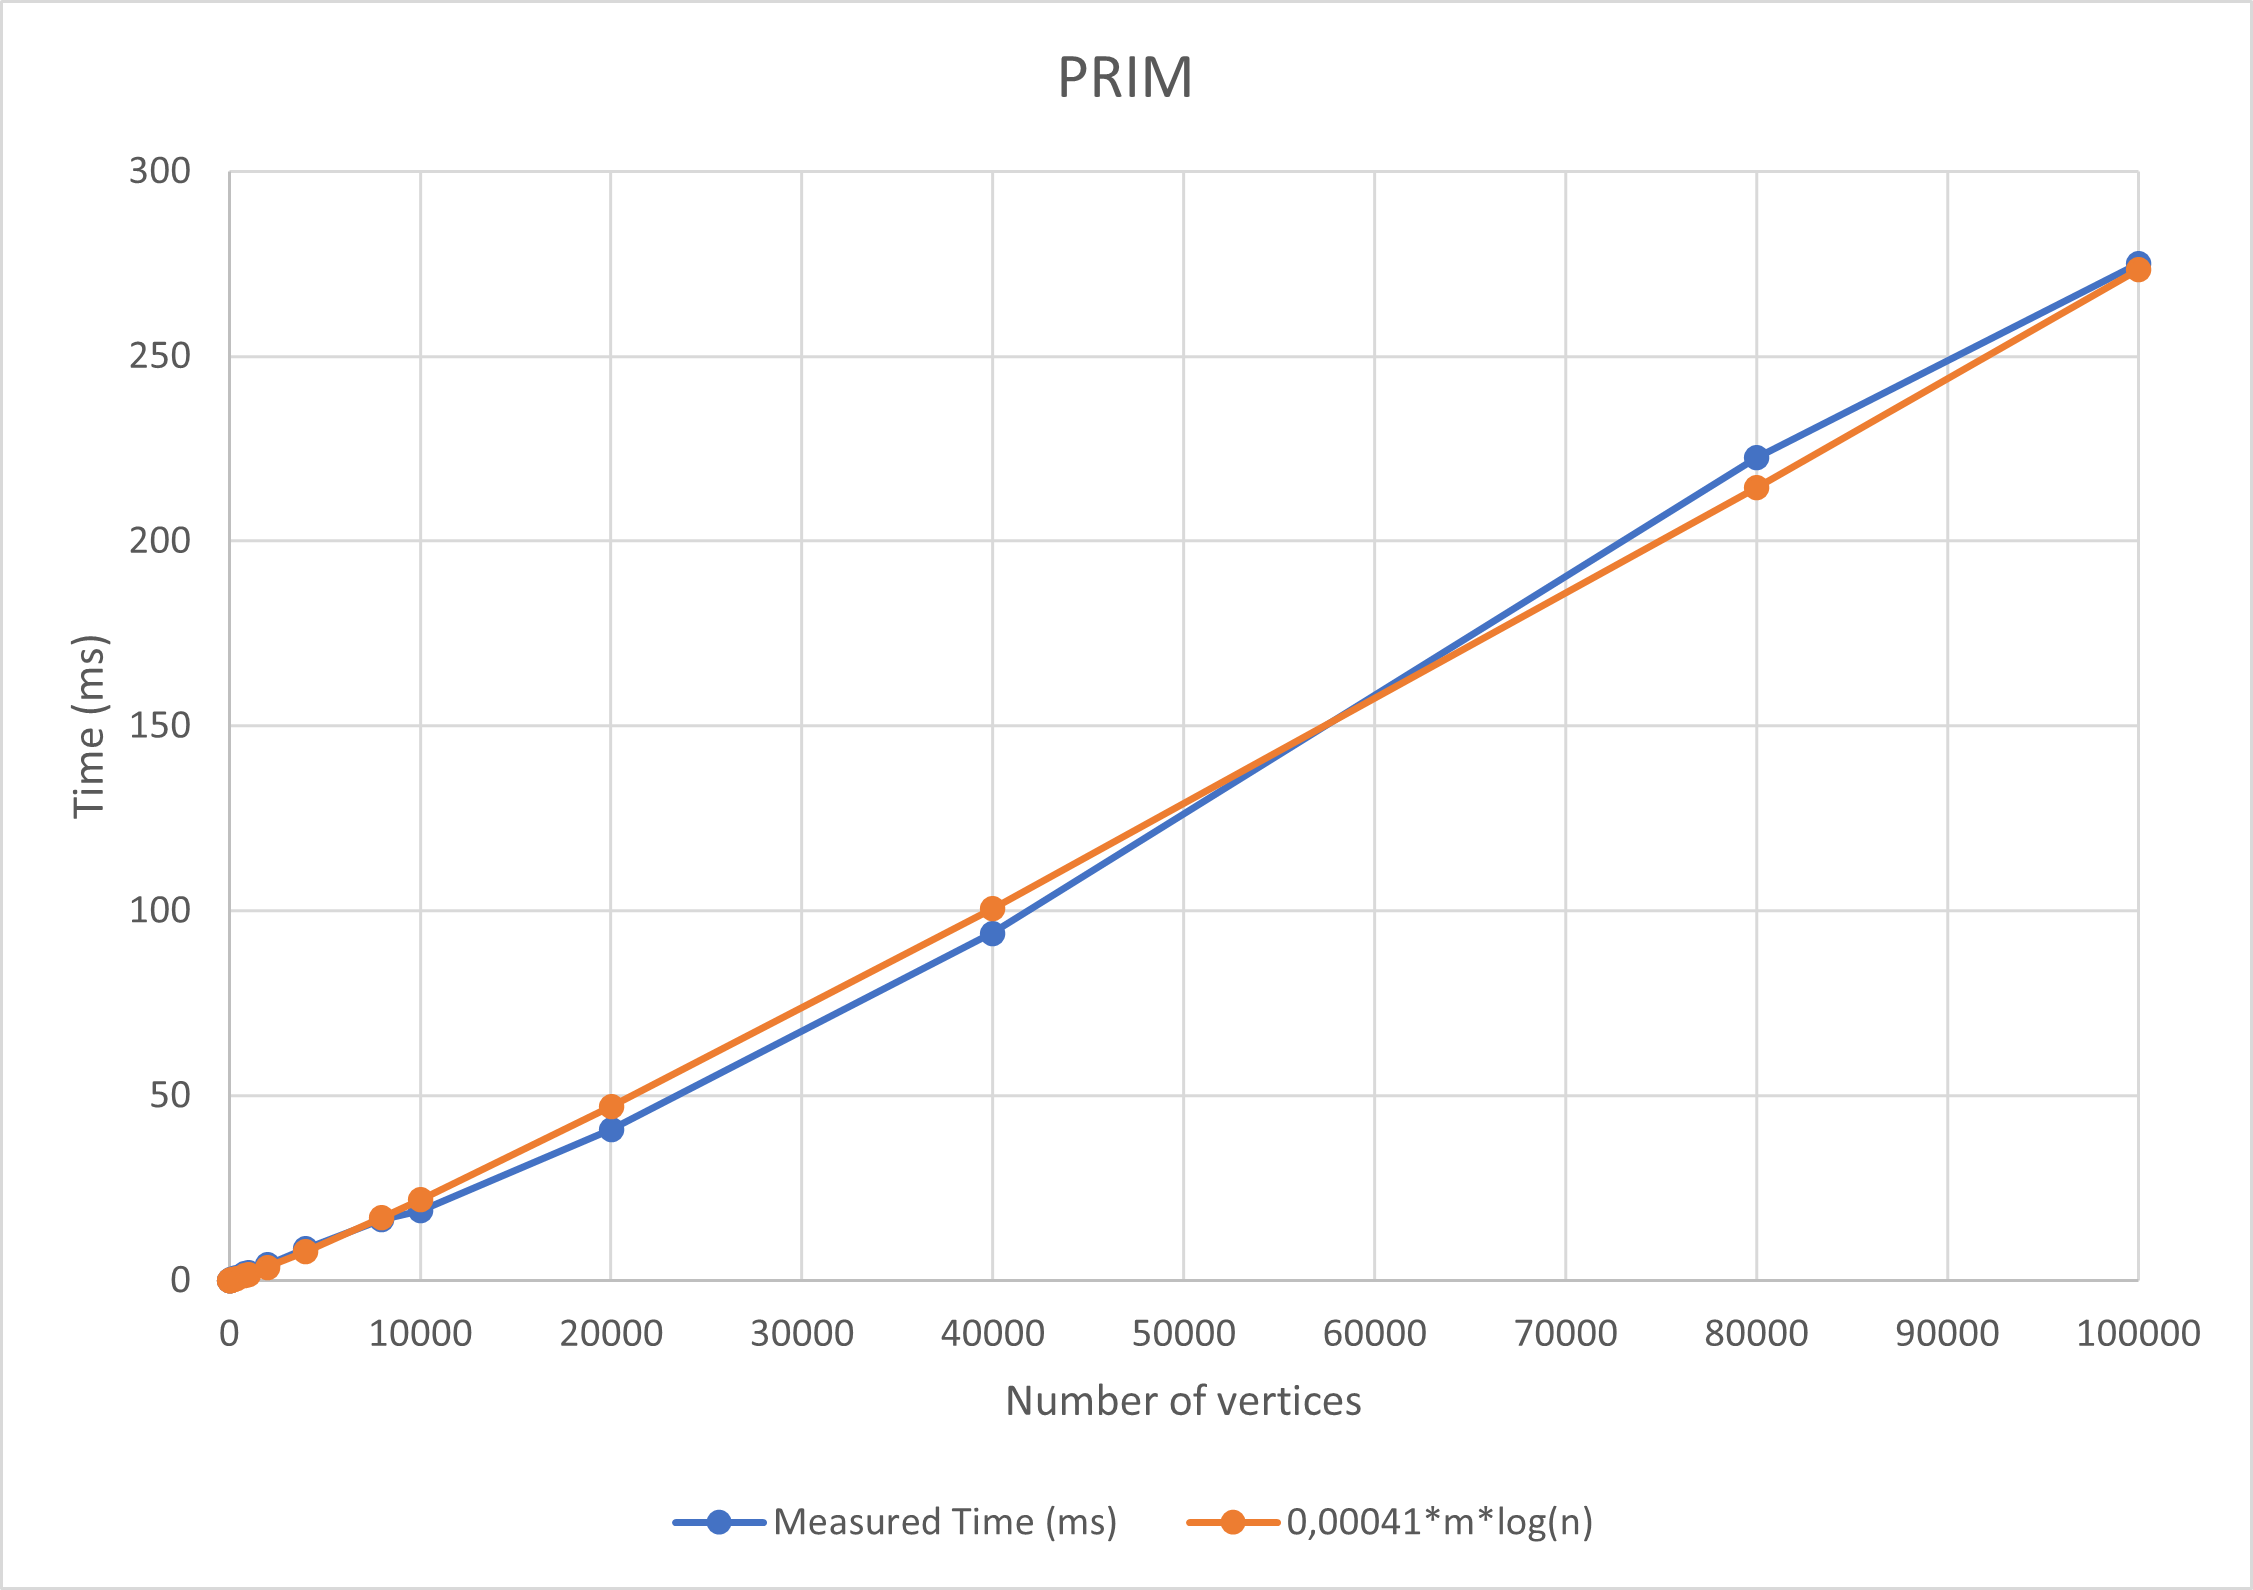
\includegraphics[width=0.8\textwidth]{../img/Prim.png}
    \caption{Prim complexity.}
    \label{fig:prim}
\end{figure}
The graph just illustrated above (fig. \ref{fig:prim}) shows the excepted (in orange) and actual (in blue) 
computational complexity for the Prim algorithm. As can be seen from the image, also in this case the actual 
complexity curve remains slightly below the theoretical curve.

\subsubsection{Results of naive Kruskal}
\begin{figure}[H]
    \centering
    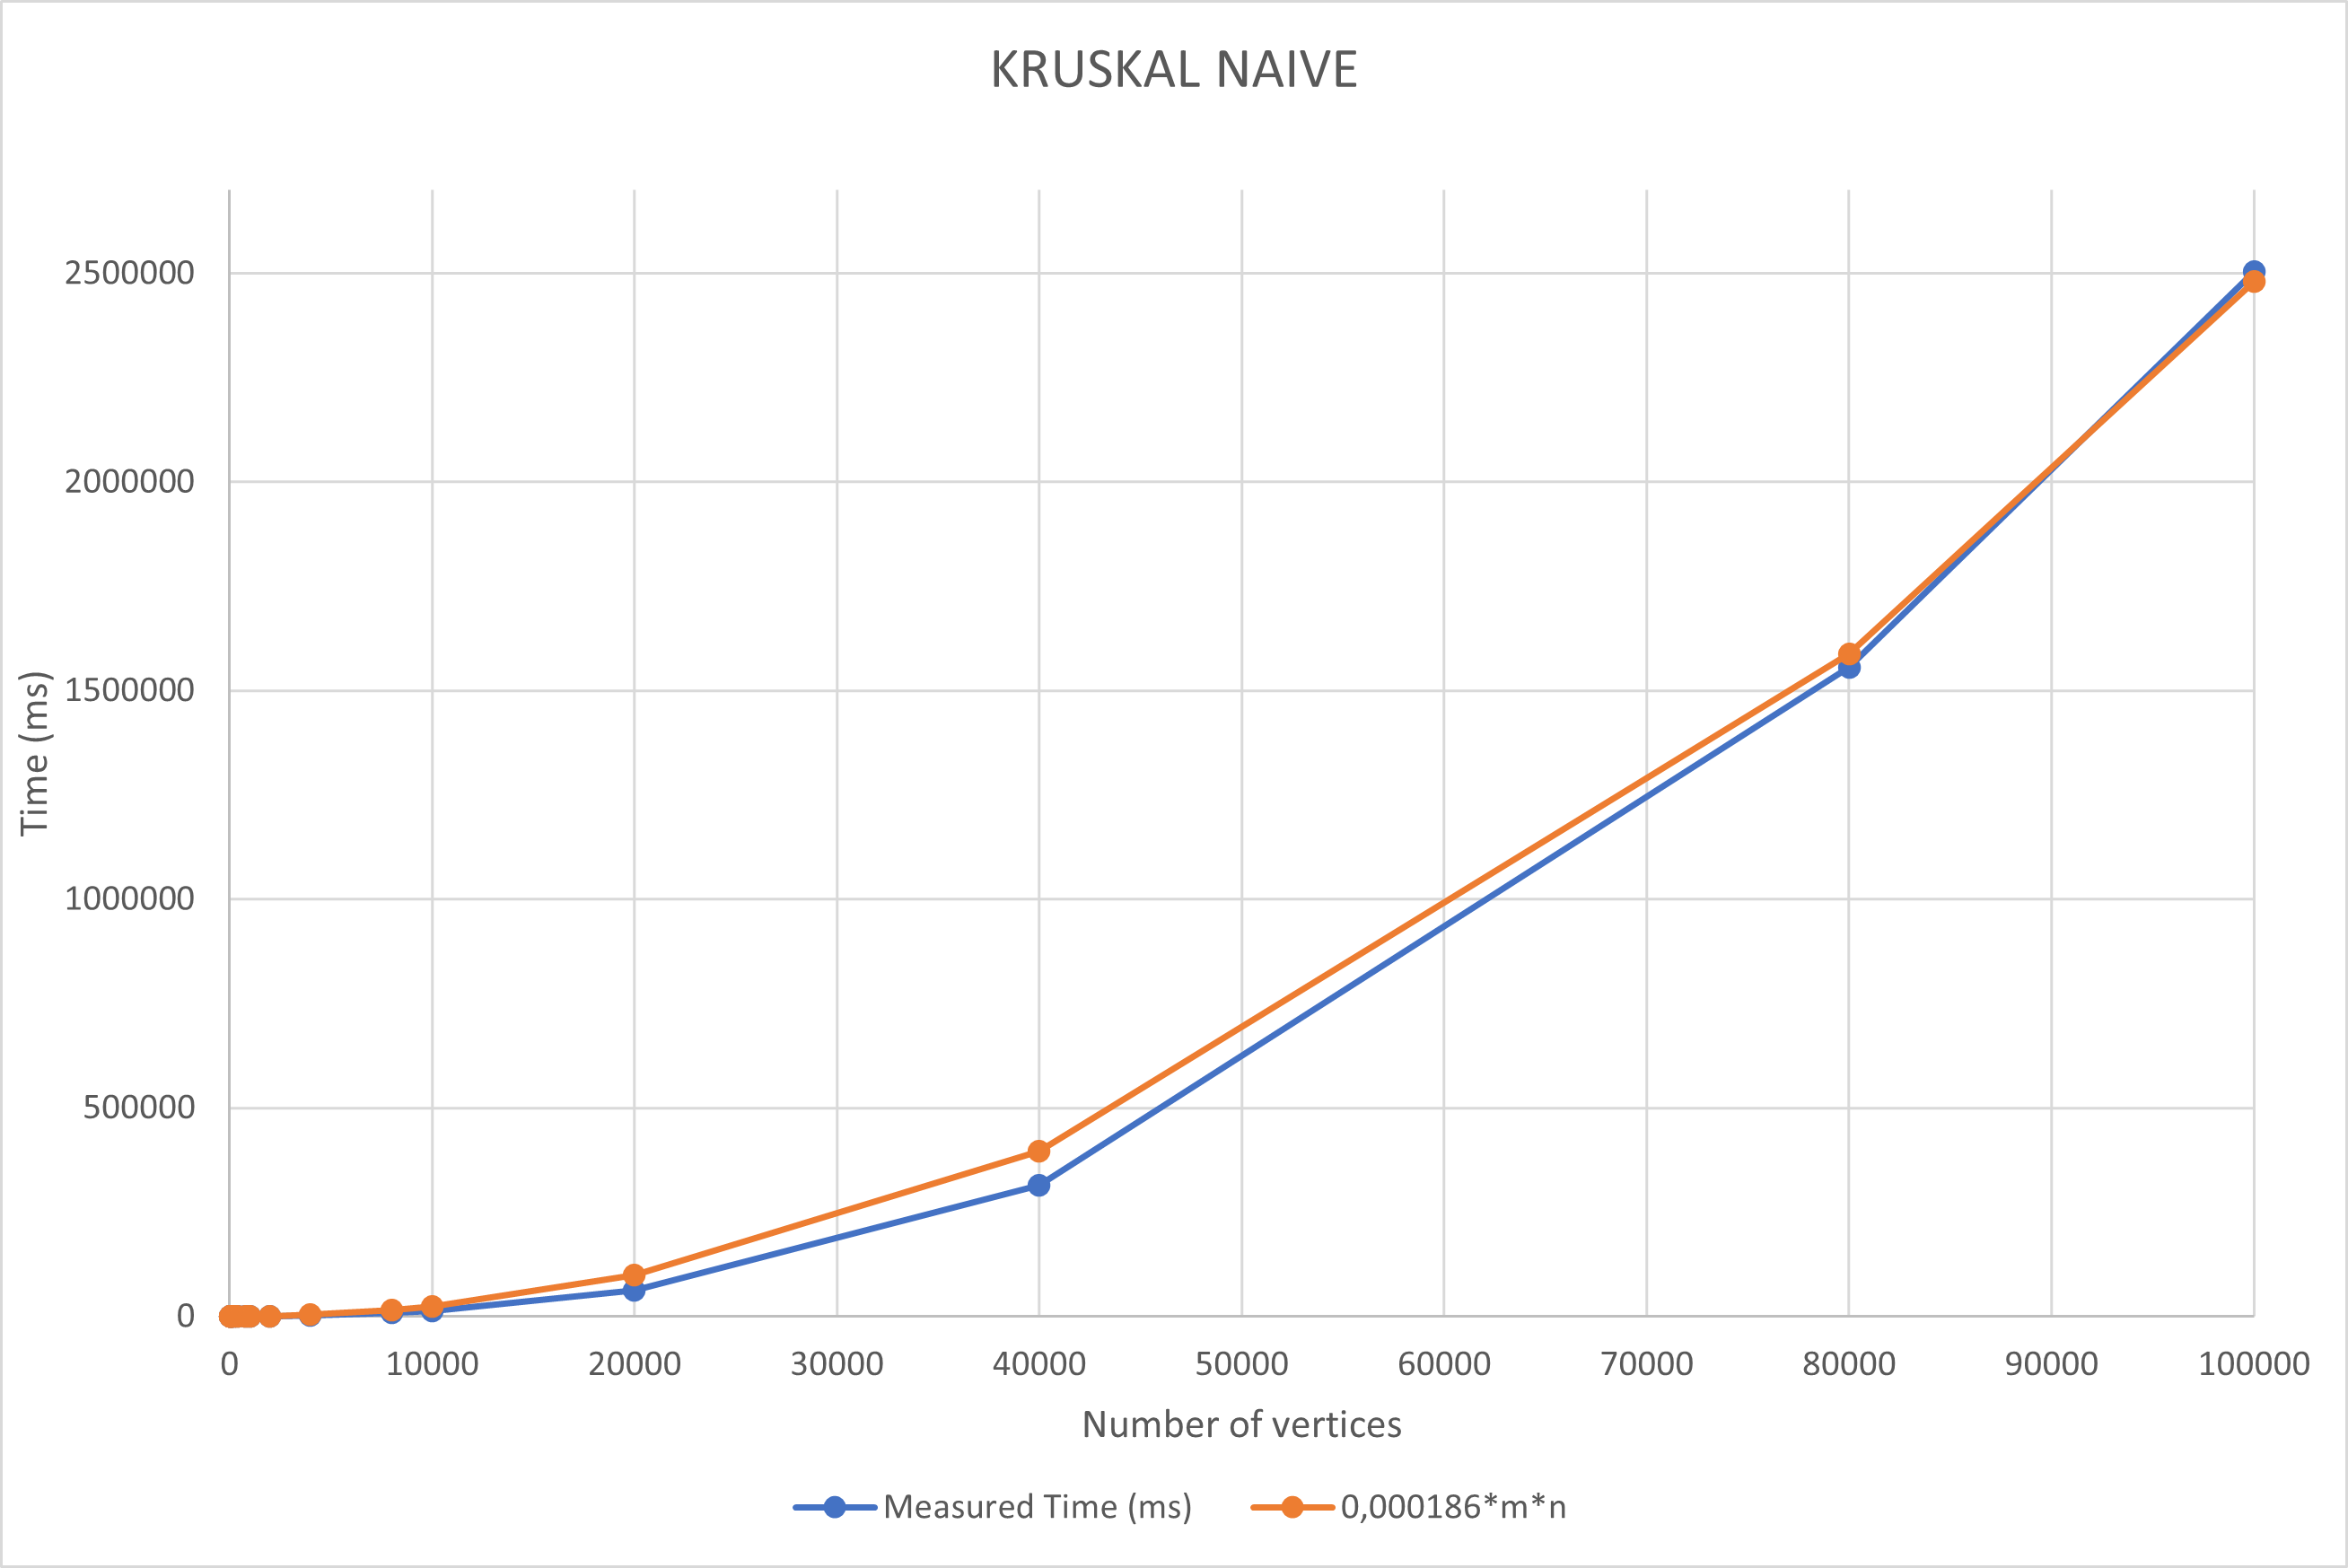
\includegraphics[width=0.8\textwidth]{../img/KruskalNaive.png}
    \caption{Naive Kruskal complexity.}
    \label{fig:kruskal}
\end{figure}
The graph just illustrated above (fig. \ref{fig:kruskal}) shows the excepted (in orange) and actual 
(in blue) computational complexity for the Kruskal Naive algorithm. As can be seen from the image, 
the actual complexity curve remains slightly below the theoretical curve and therefore the two complexities are comparable.

\subsubsection{Results of Kruskal Union Find}
\begin{figure}[H]
    \centering
    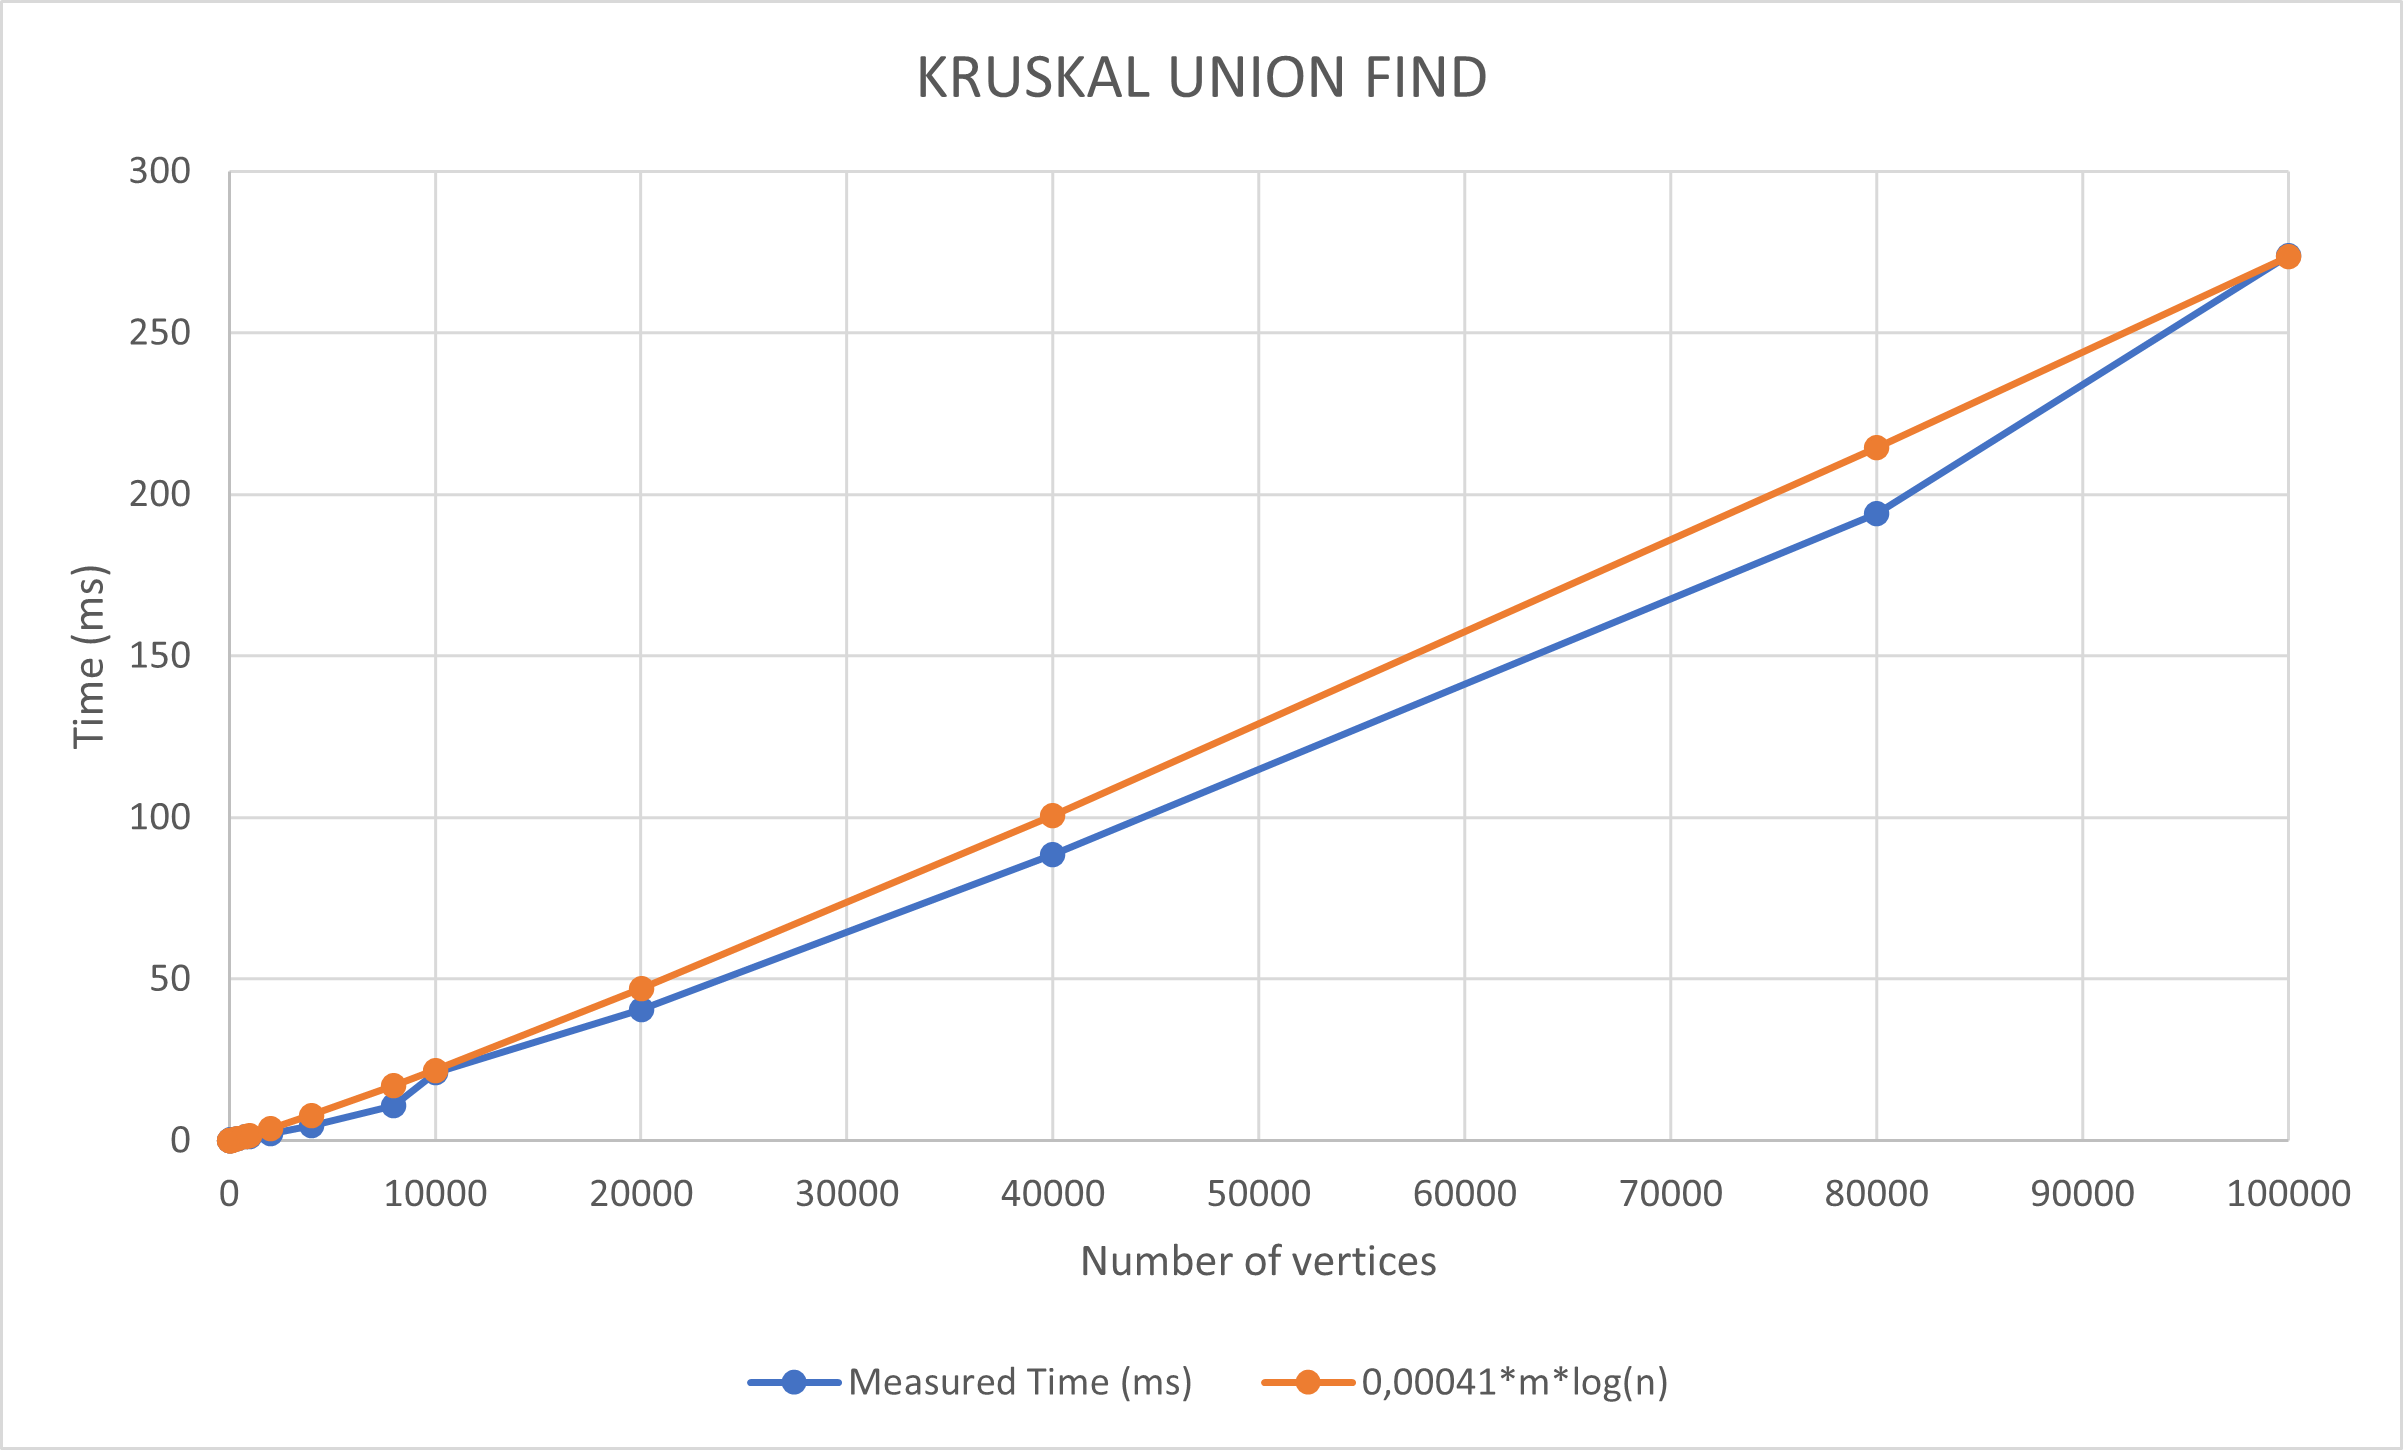
\includegraphics[width=0.8\textwidth]{../img/KruskalUnionFind.png}
    \caption{Kruskal Union Find complexity.}
    \label{fig:kruskaluf}
\end{figure}
The graph just illustrated above (fig. \ref{fig:kruskaluf}) shows the excepted (in orange) and actual 
(in blue) computational complexity for the Kruskal Union Find algorithm. In this case the actual complexity 
curve has a somewhat strange behavior, in fact for the graphs with 80000 vertices, the average time is greater than 
what it should be, but on the whole the actual complexity curve remains below the theoretical curve.

\subsection{Question 2}
\textit{Comment on the results you have obtained: how do the algorithms behave with respect to the various 
instances? There is an algorithm that is always better than the others? Which of the three algorithms you 
have implemented is more efficient?} \\

\noindent
Analyzing the three algorithms we have found that in the case of Kruskal Naive the algorithm requires a 
significantly higher average execution time than in Kruskal Union-Find and Prim. In fact, the average time 
calculated in the case of the four files containing the greatest number of vertices (100000) the results 
were as follows:
\begin{table}[H]\centering
    \begin{tabular}{l|l|l|l|l}
        \textbf{Nodes} & \textbf{Datasets} & \textbf{Prim [ms]} & \textbf{Kruskal naive [ms]} & \textbf{Kruskal U-F [ms]}\\
    \hline
        100000 & 65, 66, 67, 68 & 86.14 & 2504591,06 & 110,66 
    \end{tabular}
\end{table}
\noindent
Comparing the results of the graphs with a smaller number of vertices we could see the following:
\begin{table}[H]\centering
    \begin{tabular}{l|l|l|l|l}
        \textbf{Nodes} & \textbf{Datasets} & \textbf{Prim [ms]} & \textbf{Kruskal naive [ms]} & \textbf{Kruskal Union-Find [ms]} \\
    \hline
    %   10 & 1, 2, 3, 4     & 0,009  & 0,07  & 0,018  \\
        10 & 1, 2, 3, 4     & 0,009  & 1,73  & 0,018  \\
    %   20 & 5, 6, 7, 8     & 0,013  & 0,13  & 0,016  \\
        20 & 5, 6, 7, 8     & 0,996  & 0,13  & 1,45   \\
        40 & 9, 10, 11, 12  & 0,026  & 0,34  & 0,028  \\
    \end{tabular}
\end{table}
\noindent
Omitting some particular cases for Kruskal with Union-Find and Prim which considerably reaise the average 
time; the measured times detected with Krusal Naive are closer to the other algorithms since, working with 
a smaller amount of vertices, it is not possible to see a difference in the average execution times.

\subsubsection{Comparison Prim-Kruskal Union Find}
\begin{figure}[H]
    \centering
    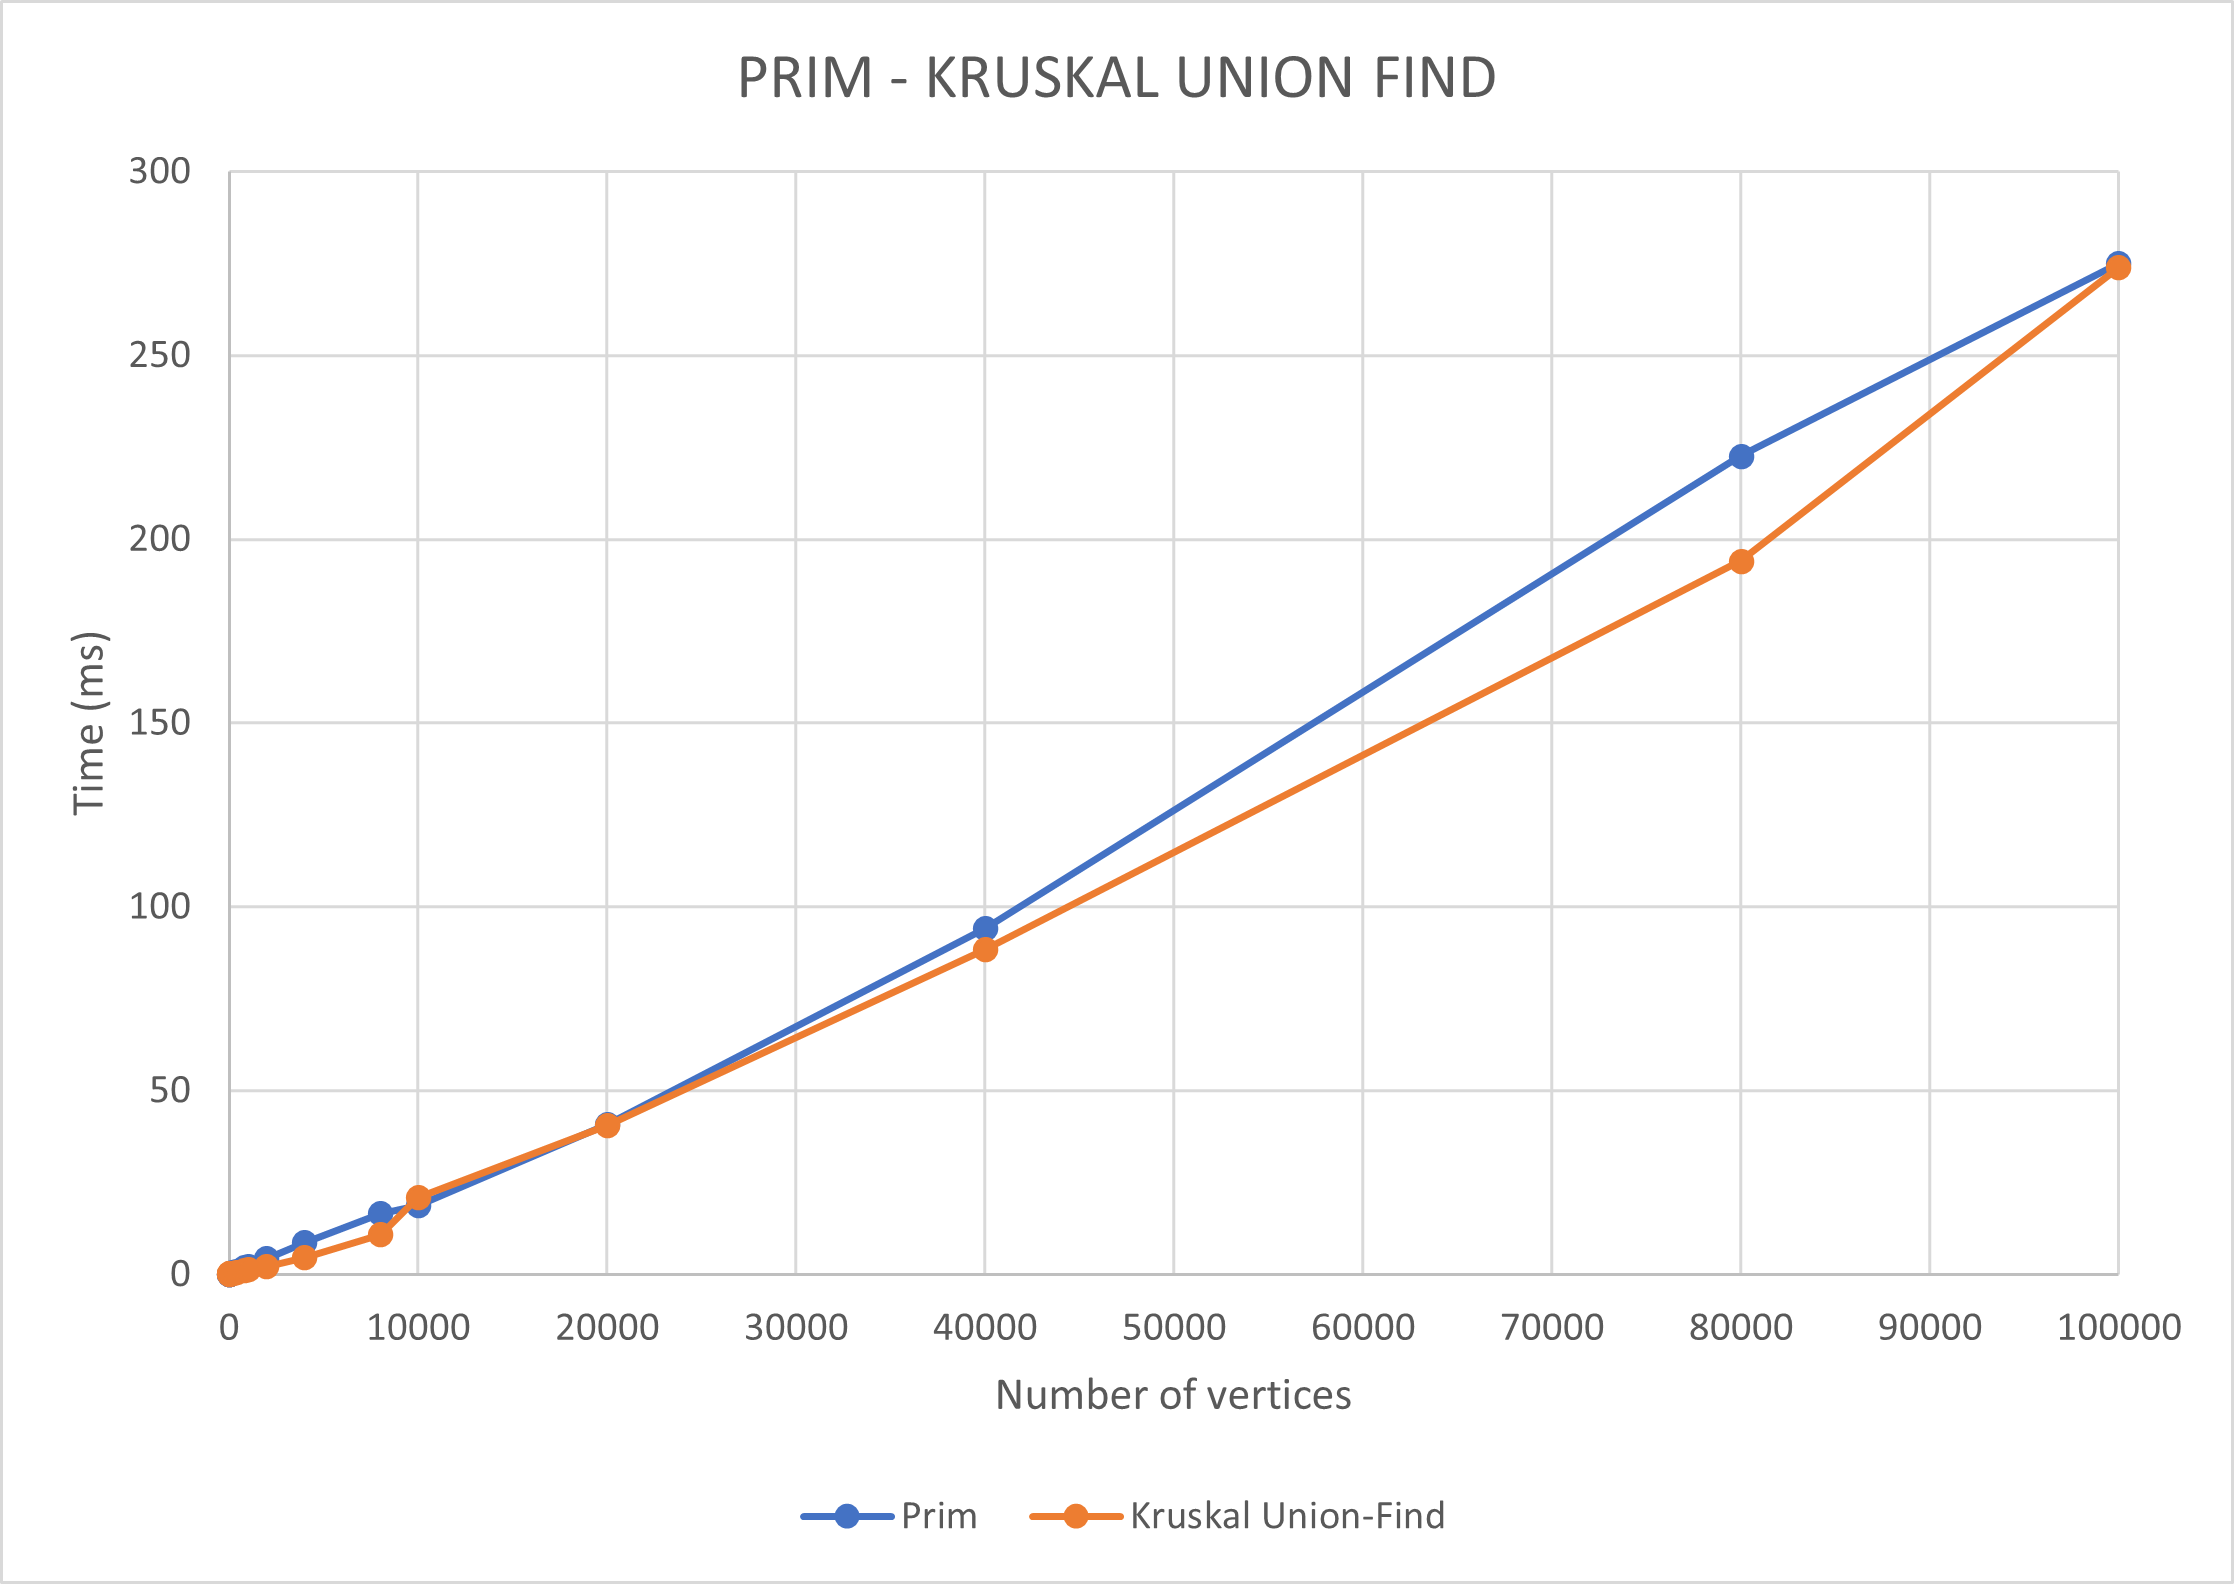
\includegraphics[width=0.8\textwidth]{../img/ComparisonPrimKruskal.png}
    \caption{Comparison between Prim and Kruskal Union-Find.}
    \label{fig:comparison}
\end{figure}
In the graph just illustrated (fig. \ref{fig:comparison}) there is a comparison between the Prim algorithm 
and Kruskal Union-Find algorithm. It can be clearly seen that \textbf{Prim algorithm turns out to be more 
efficient than Kruskal Union-Find algorithm}, since the average running time is moderately lower for Prim 
in our implementation. Therefore, from this we can conclude that the Prim algorithm always tends to do 
better than the others.